\documentclass[crop]{standalone}

\usepackage[usenames,dvipsnames]{xcolor}
\usepackage{tikz}

\usetikzlibrary{arrows,positioning}
\tikzset{>=stealth}

\begin{document}

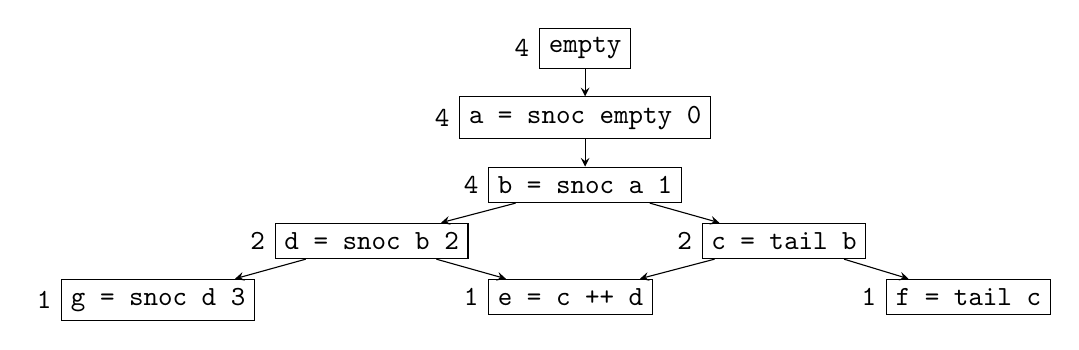
\begin{tikzpicture}[every node/.style={font=\ttfamily, rectangle, draw, thin, node distance=1em}]
  \node (empty) [label=180:{4}] {empty};
  \node (a) [below=of empty, label=180:{4}] {a = snoc empty 0};
  \node (b) [below=of a, label=180:{4}] {b = snoc a 1};
  \node (c) [below right=of b, label=180:{2}] {c = tail b};
  \node (d) [below left=of b, label=180:{2}] {d = snoc b 2};
  \node (e) [below right=of d, label=180:{1}] {e = c ++ d};
  \node (f) [below right=of c, label=180:{1}] {f = tail c};
  \node (g) [below left=of d, label=180:{1}] {g = snoc d 3};

  \draw[->] (empty) to (a);
  \draw[->] (a) to (b);
  \draw[->] (b) to (c);
  \draw[->] (b) to (d);
  \draw[->] (c) to (e);
  \draw[->] (c) to (f);
  \draw[->] (d) to (e);
  \draw[->] (d) to (g);
\end{tikzpicture}

\end{document}
